\documentclass{standalone}
\usepackage{pgfplots}
\usepackage{xspace}
\usepackage{tikz}
\usetikzlibrary{plotmarks}
\usetikzlibrary{arrows, automata, shapes.geometric, positioning}

\pgfplotsset{width=3cm, compat=1.15}


\begin{document}
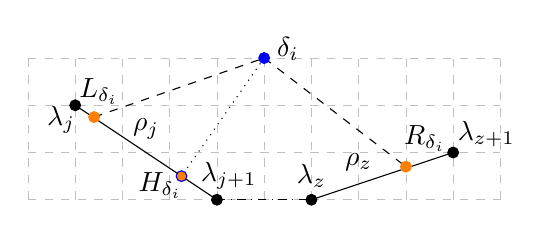
\begin{tikzpicture}[scale=0.6, every node/.style={scale=1}]
	%%%% delivery area 
	\draw[help lines, color=gray!50, dashed] (0,0) grid (10, 3);
	
	\draw[black,fill=black] (1,2) circle (.75ex);
	\draw[black,fill=black] (4,0) circle (.75ex);
	\draw[black,fill=black] (6,0) circle (.75ex);
	\draw[black,fill=black] (9,1) circle (.75ex);
	
	\draw[-] (1,2)--(4,0);
	\draw[dashdotted] (4,0)--(6,0);
	\draw[-] (6,0)--(9,1);

	\node at (2.5,1.5) {$\rho_j$};
	\node at (7,0.8) {$\rho_z$};
	%%%%%%

	


	
	
	\draw[-, dashed] (1.4,1.75)--(5,3);
	\draw[-, dashed] (5,3)--(8,0.7);

	\draw[orange,fill=orange] (1.4,1.75) circle (.75ex);
	\draw[orange,fill=orange] (8,0.7) circle (.75ex);
	
	
	\node at (1.5,2.3) {$L_{\delta_i}$};
	\node at (8.4,1.3) {$R_{\delta_i}$};

	\draw[dotted] (5,3)--(3.25,0.5);
	\draw[blue,fill=orange] (3.25,0.5) circle (.75ex);
	\node at (2.8,0.3) {$H_{\delta_i}$};
%	\node at (4,0) {$\delta_i^P$};
	
%	\node at (4.35,1.5) {$\tau_i^j$};
	
 	%%%delivery point
	\draw[blue,fill=blue] (5,3) circle (.75ex);
	\node at (5.5,3.2) {$\delta_i$};
	\node at (0.7,1.7) {$\lambda_j$};
	\node at (4.25,0.5) {$\lambda_{j+1}$};
	\node at (6,0.5) {$\lambda_z$};
	\node at (9.7,1.4) {$\lambda_{z+1}$};
	%%%%%%%
\end{tikzpicture}
\end{document}